\documentclass[a4paper,twoside]{article}
\usepackage{blindtext}  
\usepackage{geometry}

% Chinese support
\usepackage[UTF8, scheme = plain]{ctex}

% Page margin layout
\geometry{left=2.3cm,right=2cm,top=2.5cm,bottom=2.0cm}


\usepackage{listings}
\usepackage{xcolor}
\usepackage{geometry}
\usepackage{amsmath}
\usepackage{float}
\usepackage{hyperref}

\usepackage{graphics}
\usepackage{graphicx}
\usepackage{subfigure}
\usepackage{epsfig}
\usepackage{float}

\usepackage{algorithm}
\usepackage[noend]{algpseudocode}

\usepackage{booktabs}
\usepackage{threeparttable}
\usepackage{longtable}
\usepackage{listings}

% cite package, to clean up citations in the main text. Do not remove.
\usepackage{cite}

\usepackage{color,xcolor}

%% The amssymb package provides various useful mathematical symbols
\usepackage{amssymb}
%% The amsthm package provides extended theorem environments
\usepackage{amsthm}
\usepackage{amsfonts}
\usepackage{enumerate}
\usepackage{enumitem}
\usepackage{listings}

\usepackage{indentfirst}
\setlength{\parindent}{2em} % Make two letter space in the first paragraph
\usepackage{setspace}
\linespread{1.5} % Line spacing setting
\usepackage{siunitx}
\setlength{\parskip}{0.5em} % Paragraph spacing setting

% \usepackage[contents =22920202204622, scale = 10, color = black, angle = 50, opacity = .10]{background}

\renewcommand{\figurename}{图}
\renewcommand{\lstlistingname}{代码} 
\renewcommand{\tablename}{表格}
\renewcommand{\contentsname}{目录}
\floatname{algorithm}{算法}

\graphicspath{ {images/} }

%%%%%%%%%%%%%
\newcommand{\StudentNumber}{22920202204622}  % Fill your student number here
\newcommand{\StudentName}{熊恪峥}  % Replace your name here
\newcommand{\PaperTitle}{实验(一) \ 实现三次样条插值}  % Change your paper title here
\newcommand{\PaperType}{计算方法(A)} % Replace the type of your report here
\newcommand{\Date}{2022年3月11日}
\newcommand{\College}{信息学院}
\newcommand{\CourseName}{计算方法(A)}
%%%%%%%%%%%%%

%% Page header and footer setting
\usepackage{fancyhdr}
\usepackage{lastpage}
\pagestyle{fancy}
\fancyhf{}
% This requires the document to be twoside
\fancyhead[LO]{\texttt{\StudentName }}
\fancyhead[LE]{\texttt{\StudentNumber}}
\fancyhead[C]{\texttt{\PaperTitle }}
\fancyhead[R]{\texttt{第{\thepage}页,共\pageref*{LastPage}页}}


\title{\PaperTitle}
\author{\StudentName}
\date{\Date}

\lstset{
	basicstyle          =   \sffamily,          % 基本代码风格
	keywordstyle        =   \bfseries,          % 关键字风格
	commentstyle        =   \rmfamily\itshape,  % 注释的风格,斜体
	stringstyle         =   \ttfamily,  % 字符串风格
	flexiblecolumns,                % 别问为什么,加上这个
	numbers             =   left,   % 行号的位置在左边
	showspaces          =   false,  % 是否显示空格,显示了有点乱,所以不现实了
	numberstyle         =   \zihao{-5}\ttfamily,    % 行号的样式,小五号,tt等宽字体
	showstringspaces    =   false,
	captionpos          =   t,      % 这段代码的名字所呈现的位置,t指的是top上面
	frame               =   lrtb,   % 显示边框
}

\lstdefinestyle{PythonStyle}{
	language        =   Python, % 语言选Python
	basicstyle      =   \zihao{-5}\ttfamily,
	numberstyle     =   \zihao{-5}\ttfamily,
	keywordstyle    =   \color{blue},
	keywordstyle    =   [2] \color{teal},
	stringstyle     =   \color{magenta},
	commentstyle    =   \color{red}\ttfamily,
	breaklines      =   true,   % 自动换行,建议不要写太长的行
	columns         =   fixed,  % 如果不加这一句,字间距就不固定,很丑,必须加
	basewidth       =   0.5em,
}

\lstdefinestyle{MatlabStyle}{
	language        =   Matlab, 
	keywordstyle    =   \color{blue},
	keywordstyle    =   [2] \color{teal},
	stringstyle     =   \color{magenta},
	commentstyle    =   \color{red}\ttfamily,
	breaklines      =   true,
	columns         =   fixed,
	basewidth       =   0.5em,
}

\begin{document}
	
%%%%%%%%%%%%%%%%%%%%%%%%%%%%%%%%%%%%%%%%%%%%
\makeatletter % change default title style
\renewcommand*\maketitle{%
	\begin{center} 
		\bfseries  % title 
		{\LARGE \@title \par}  % LARGE typesetting
		\vskip 1em  %  margin 1em
		{\global\let\author\@empty}  % no author information
		{\global\let\date\@empty}  % no date
		\thispagestyle{empty}   %  empty page style
	\end{center}%
	\setcounter{footnote}{0}%
}
\makeatother
%%%%%%%%%%%%%%%%%%%%%%%%%%%%%%%%%%%%%%%%%%%%
	
	
\thispagestyle{empty}

\vspace*{1cm}

\begin{figure}[h]
	\centering
	
\includegraphics[width=4.0cm]{logo.png}
\end{figure}

\vspace*{1cm}

\begin{center}
	\Huge{\textbf{\PaperType}}
	
	\Large{\PaperTitle}
\end{center}

\vspace*{1cm}

\begin{table}[h]
	\centering	
	\begin{Large}
		\renewcommand{\arraystretch}{1.5}
		\begin{tabular}{p{3cm} p{5cm}<{\centering}}
			姓\qquad 名 & \StudentName  \\
			\hline
			学\qquad号 & \StudentNumber \\
			\hline
			日\qquad期 & \Date  \\
			\hline
			学\qquad院 & \College  \\
			\hline
			课程名称 & \CourseName  \\
			\hline
		\end{tabular}
	\end{Large}
\end{table}

\newpage

\title{
	\Large{\textcolor{black}{\PaperTitle}}
}
	
	
\maketitle
	
\tableofcontents
 
\newpage
\begin{spacing}{1.2}

\section{项目结构}
\label{sec:struct}

本程序(\textbf{以下称为pyCSI})的目录结构如表\ref{tbl:codestruct}。pyCSI使用Python完成,只使用了最低限度的、必要的第三方库来进行运算的优化和符号计算的处理。该项目是高度结构化的。因为各种约束的三弯矩方程的系数矩阵有很多相似之处,并且不同约束条件的三次样条插值求解有很多的相同部分,因此pyCSI把这些部分抽象成单独的函数,并且放在不同的文件中,提高了代码的可读性,最后提供一个统一的接口$pyCSI.spline$,方便在其他需要执行三次样条插值的代码中直接调用。

\begin{table}[h]
	\caption{代码文件结构}
	\label{tbl:codestruct}
	\begin{center}
		\begin{tabular}{p{5cm}p{8cm}}
			\toprule
			路径 & 功能 \\
			\midrule
			main.py & 调用$pyCSI.spline$进行测试和可视化 \\
			\hline
			pyCSI/spline.py & 提供本程序实现的对外接口$pyCSI.spline$ \\
			\hline
			pyCSI/impl/derivative1.py, pyCSI/impl/derivative2.py, pyCSI/impl/notaknot.py,  pyCSI/impl/periodic.py & 分别实现了一阶导数约束、二阶导数约束、非扭结(Not-A-Knot)约束、周期函数约束的三次样条插值 \\
			\hline
			pyCSI/impl/preprocess.py & 实现了对三弯矩方程矩阵构建的预处理,因为各种约束条件的三弯矩矩阵都有较为相似的部分 \\
			\hline
			pyCSI/impl/thomas.py & 实现了Thomas Algorithm(追赶法)解三对角矩阵的线性方程组 \\
			\hline
			pyCSI/impl/thomas.py & 实现了一些帮助函数,用来构建输出的系数矩阵或者SymPy分段符号函数,以及通过对角线向量构建三对角矩阵 \\
			\bottomrule
		\end{tabular}
	\end{center}
\end{table}

pyCSI主要依赖两个第三方库:

\begin{itemize}
	\item \textbf{NumPy} Python的科学计算库,提供了对向量和矩阵高效的计算操作
	\item \textbf{SymPy} Python的符号计算库,提供了符号计算的能力,主要用于输出符号函数和绘图
\end{itemize}

\section{项目实现}

pyCSI为三次样条插值提供了统一的接口,有如下参数
\begin{lstlisting}[language=Python,numbers=left,style=PythonStyle,label={code:interface}]
def spline(x: Iterable, y: Iterable, constraint_type: ConstraintType = ConstraintType.NOT_A_KNOT,
symbolic_result: bool = True, **constraints):
\end{lstlisting}

\begin{itemize}
	\item \textbf{x,y} 插值点的$x$,$y$值
	\item \textbf{constriant\_type} 要使用的约束类型,支持一阶导数、二阶导数、自然约束(二阶导数为0)、非扭结约束、周期函数约束
	\item \textbf{symbolic\_result} 为$true$返回一个SymPy符号函数,是插值得到的分段函数,否则返回三次样条插值函数中每一项的系数组成的矩阵
	\item \textbf{constraints} 额外给定的约束(如果需要)。当使用一阶导数约束时需要给定$m0$和$mn$,使用二阶导约束时需要给定$M0$和$Mn$,否则会抛出运行时异常
\end{itemize}

具体实现以一阶导数约束的实现为例,如代码\ref{code:d1},首先预处理出三对角矩阵的三条对角线,以NumPy向量的形式,然后根据给定的参数填入一阶导约束独有的部分,最后构建三弯矩方程并使用追赶法求解,最后计算插值函数每一个括号前的系数。该结果返回给$pyCSI.spline$后它会决定直接返回还是进一步构建一个SymPy符号函数。具体的预处理和求解都是按照公式实现的,\textbf{具体实现请参见相关代码文件}。\nameref{sec:appB}给出了追赶法解方程的代码实现,如代码\ref{code:thomas}

\begin{lstlisting}[language=Python,numbers=left,style=PythonStyle,caption=一阶导数约束的实现,label={code:d1}]
def spline_impl_derive1(x: np.ndarray, y: np.ndarray, h: np.ndarray, m0: np.float, mn: np.float):
	N: Final = x.shape[0] - 1
	
	alpha, beta, c, dy = preprocess_args(y, h, N)
	
	# by constraint
	alpha[N] = 1
	beta[0] = 1
	c[0] = (6.0 / h[0]) * (dy[0] / h[0] - m0)
	c[N] = (6.0 / h[N - 1]) * (dy[N - 1] / h[N - 1] + mn)
	
	M: Final = thomas_solve(alpha[1:N + 1], 2 * np.ones(N + 1), beta[0:N], c)

	return calculate_coefficients(M, y, h, N)
\end{lstlisting}



以函数$y=\frac{1}{1+x^2} \ x \in [-5,5]$为例,使用非扭结约束插值,输出SymPy符号函数,输出的函数如下,是已经打开括号并化简过的表达式。如果选择输出系数矩阵,输出的并不是该分段函数每一项的系数,而是按照书上给出的三次样条函数标准形式每一个括号前的系数。

\begin{lstlisting}[language=Python,numbers=left,style=PythonStyle,caption=输出的结果,label={code:d1}]
Piecewise((0.00646792653713069*x**2 + 0.0785733297844025*x + 0.269630023955284, (x >= -5) & (x < -4)), (0.00787862656374767*x**3 + 0.101011445302103*x**2 + 0.456747404844291*x + 0.773862124035135, (x >= -4) & (x < -3)), (0.00649454351876496*x**3 + 0.0885546978972584*x**2 + 0.419377162629758*x + 0.736491881820602, (x >= -3) & (x < -2)), (0.107319669949428*x**3 + 0.693505456481235*x**2 + 1.62927867979771*x + 1.5430928932659, (x >= -2) & (x < -1)), (-0.435773223316476*x**3 - 0.935773223316476*x**2 + 1, (x >= -1) & (x < 0)), (0.435773223316476*x**3 - 0.935773223316476*x**2 + 1.11022302462516e-16*x + 1, (x >= 0) & (x < 1)), (-0.107319669949428*x**3 + 0.693505456481235*x**2 - 1.62927867979771*x + 1.5430928932659, (x >= 1) & (x < 2)), (-0.00649454351876498*x**3 + 0.0885546978972585*x**2 - 0.419377162629758*x + 0.736491881820602, (x >= 2) & (x < 3)), (-0.00787862656374766*x**3 + 0.101011445302103*x**2 - 0.45674740484429*x + 0.773862124035134, (x >= 3) & (x < 4)), (0.0064679265371307*x**2 - 0.0785733297844025*x + 0.269630023955284, (x >= 4) & (x < 5)))
\end{lstlisting}


对它进行作图,得到图\ref{fig:result},可以看出插值效果是正确的。

\begin{figure}[h]
	\centering
	\caption{插值结果}
	\label{fig:result}
	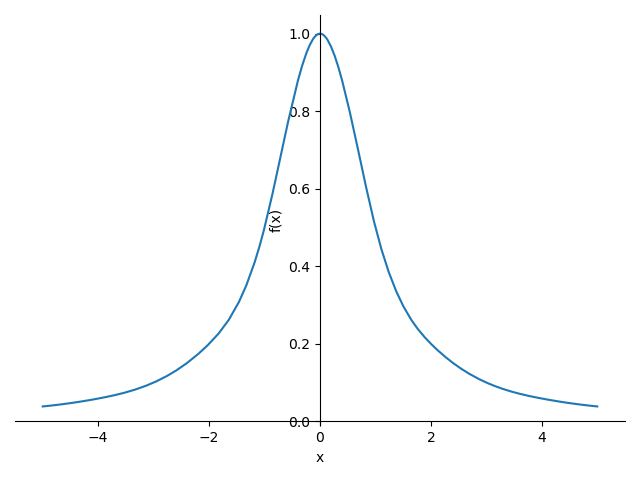
\includegraphics[width=0.5\linewidth]{test.png}
\end{figure}

其他插值约束的实现见相关文件,插值效果都经过测试,是正确的。需要注意到的是建立符号函数时展开、化简多项式需要的时间较多,因此返回系数矩阵能大大加快运行速度。

\section{基准测试}

本程序(\textbf{以下称为pyCSI})在性能方面表现较好。以Matlab R2021b为基线进行测试\footnote{测试环境: i7-10800H, RTX3060, 32GB运行内存的便携式计算机,运行Windows 11},在点数不多的情况下,该程序性能有显著优势。运行时长随点数增加呈线性增长,增长情况比较稳定,如图\ref{fig:runtimeton}。测试代码见\nameref{sec:appA},测试数据基本情况如下

\begin{itemize}
	\item 测试函数: $y=\frac{1}{1+x^2} \ \ \ x \in [-5,5]$
	\item 点数范围: 等距取10到100个点
	\item 测量方法: 计算一百次插值计时间平均数,排除系统波动影响
	\item Matlab使用interp1函数,pyCSI使用输出各项系数的参数调用$pyCSI.spline$
\end{itemize}

\begin{figure}[h]
	\caption{单次调用平均时间$t$随插值点数$n$变化曲线图}
	
	\subfigure[pyCSI]{
		\begin{minipage}[t]{0.54\linewidth}
			\centering
			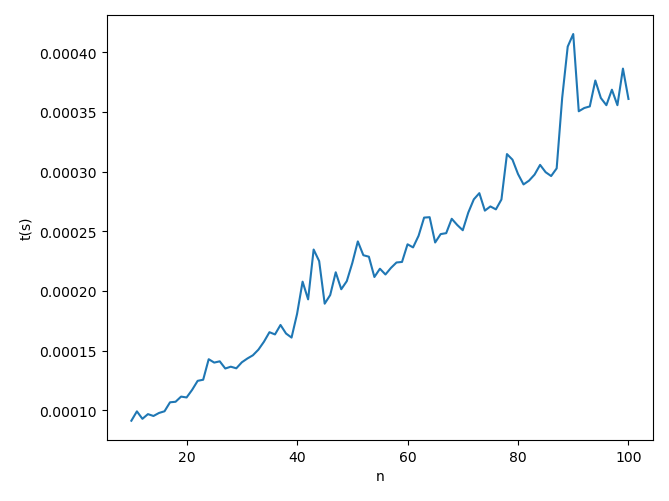
\includegraphics[width=\textwidth]{runtime/csi.png}
	\end{minipage}}
	\subfigure[Matlab]{
		\begin{minipage}[t]{0.5\linewidth}
			\centering
			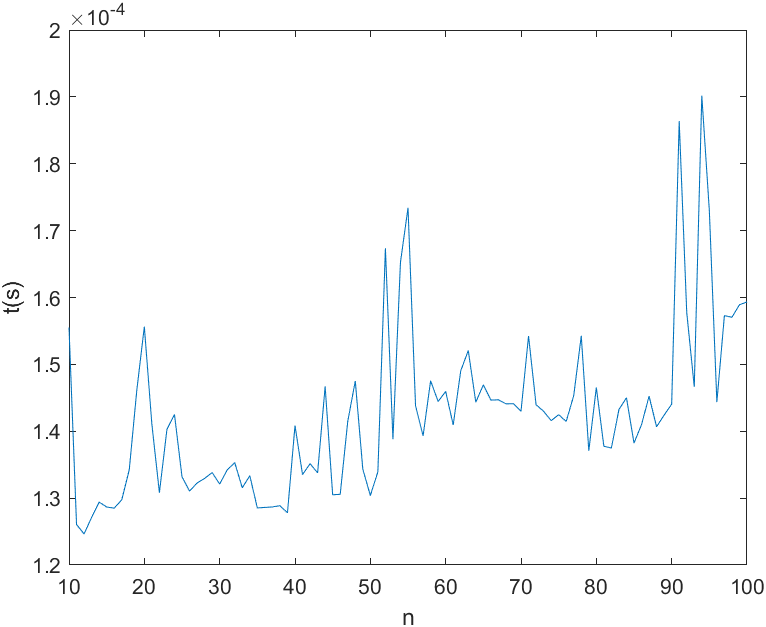
\includegraphics[width=\textwidth]{runtime/matlab.png}
	\end{minipage}}
	
	\label{fig:runtimeton}
\end{figure}

计算图\ref{fig:runtimeton}中测试运行时间的平均值,如图\ref{fig:rubtimeaverage}。本程序平均比Matlab慢仅$51.39 \%$,考虑到在规模较低的范围内($n\le40$)性能稳定地具有优势,可以认为该实现已经有优秀的运行效率了。

\begin{figure}[h]
	\centering
	\caption{平均运行时间}
	\label{fig:rubtimeaverage}
	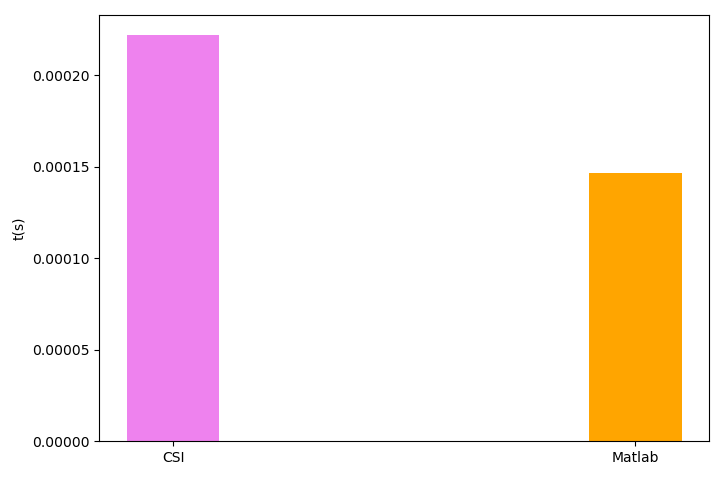
\includegraphics[width=0.5\linewidth]{average_runtime.png}
\end{figure}

进一步分析运行效率问题,通过cProfile对以上测试代码进行Profiling结果摘录前十位如表\ref{tbl:profiling},可以发现通过追赶法解三弯矩方程($thomas\_solve$)是一个性能热点,而构建三弯矩方程的矩阵($preprocess\_args$)是另一个性能热点。其他的均是Python和相关第三方库的内部函数。因此可以得出以下的结论:

\begin{itemize}
	\item Python和第三方库的内部函数对性能有较为显著的影响
	\item $thomas\_solve$和$preprocess\_args$成为性能热点是正常的,一定程度上难以继续优化,因为计算原理决定了它们需要直接在Python代码中使用循环实现,而不能使用NumPy的运算符进行表示,这意味着更多计算发生在Python代码中,而不是NumPy的实现中。后者使用C++完成,并且能够提供大量硬件相关的并行优化的支持。
\end{itemize}

\begin{table}[h]
	\begin{center}
		\caption{Profiling结果按时长排序前十位}
		\label{tbl:profiling}
		\begin{tabular}{cccc}
			\toprule 
			Name & Call Count & Time(ms) & Own Time(ms) \\
			\midrule
			thomas\_solve &	9100&	977&	953\\
			$<$built-in method \_imp.create\_dynamic$>$&	153&	922&	921\\
			preprocess\_args	&9100&	824&	659\\
			$<$built-in method io.open\_code$>$&	1247&	269&	269\\
			cleandoc&	32052&	406	&251\\
			$<$built-in method nt.stat$>$&	5424&	178	&178\\
			$<$built-in method marshal.loads$>$&	1247&	156&	156\\
			$<$method 'read' of '\_io.BufferedReader' objects$>$&	1247&	135&	135\\
			diff&	27300	&136&	120\\
			calculate\_coefficients&	9100&	139	&98\\
			\bottomrule
		\end{tabular}
	\end{center}
\end{table}


此外,可以发现pyCSI的插值用时随问题规模线性增长,而Matlab在一定范围内波动,增长较为缓慢。我推测Matlab采取的算法中某些插值规模产生的大量计算恰好和CPU的向量化寄存器大小有整数倍关系,能够使用CPU的向量化指令进行并行优化,因此对于特定规模的插值问题具有良好的性能表现。

对于较大规模的问题,我认为可能可以采用GPU来解最终的三弯矩线性方程组、进行对结果的系数等大量数据的运算。但对于一般规模,考虑到将数据传输到GPU的通信成本等开销,我认为实现GPU运算的优化并不划算。所以我没有进行相应的实现。

\clearpage
\appendix

\section{附录:测试代码}
\label{sec:appA}

该部分给出了用于基准测试的测试代码,包括Python的和Matlab的。

\begin{lstlisting}[language=Python,numbers=left,style=PythonStyle,caption=Python性能测试用代码]
import numpy as np
import sympy as sp

import matplotlib.pyplot as plt
import seaborn as sns

import timeit

import pyCSI.spline as sl


def test_func(x):
return 1 / (1 + x ** 2)
	
counts = [i for i in range(10, 101)]
times = []

for i in counts:
x = np.linspace(start=-5, stop=5, num=i)
y = np.ones(x.shape[0]) / (np.ones(x.shape[0]) + x ** 2)

start = timeit.default_timer()
for j in range(0, 100):
sl.spline(x, y, sl.ConstraintType.NOT_A_KNOT, False)
end = timeit.default_timer()

times.append((end - start) / 100.0)

average = sum(times) / len(times)
sns.lineplot(x=counts, y=times)
plt.xlabel("n")
plt.ylabel("t(s)")
plt.show()

plt.clf()

data = [average, 1.466272222222222e-04]
labels = ['pyCSI', 'Matlab']

plt.bar(range(len(data)), data, tick_label=labels, width=0.2, color=["violet", "orange"])
plt.ylabel("t(s)")
plt.show()

print(((average - 1.466272222222222e-04) / 1.466272222222222e-04)*100)
\end{lstlisting}

\newpage

\begin{lstlisting}[style=MatlabStyle,caption=Matlab性能测试用代码]
clear;
counts=10:1:100;
times=[];
total_time=0;
for count=counts
x=linspace(-5,5,count);
y=1./(1+x.^2);

tic
for i=0:1:100
pp=interp1(x,y,'spline','pp') ;
end

time=toc/100;
times=[times time];
total_time=total_time + time;

clear i
clear x
clear y
clear pp
end

plot(counts,times)
xlabel("n")
ylabel("t(s)")

total_time/90
\end{lstlisting}

\clearpage

\section{附录: 关键部分代码}
\label{sec:appB}

这里给出追赶法解三对角系数矩阵的线性方程组的代码,以及预处理系数矩阵的代码。其他代码按照\nameref{sec:struct}中的表\ref{tbl:codestruct}参见相关的代码文件

\begin{lstlisting}[language=Python,numbers=left,style=PythonStyle,caption=追赶法解方程,label={code:thomas}]
	def thomas_solve(a, b, c, d) -> np.ndarray:
	"""
	Use Thomas's algorithm to solve a tri-diagonal system
	:param a: lower diagonal
	:param b: main diagonal
	:param c: upper diagonal
	:param d: the result vector on the right of the equal sign
	:return: return the solution
	"""
	
	n = len(d)
	w = np.zeros(n - 1, float)
	g = np.zeros(n, float)
	p = np.zeros(n, float)
	
	w[0] = c[0] / b[0]
	g[0] = d[0] / b[0]
	
	for i in range(1, n - 1):
	w[i] = c[i] / (b[i] - a[i - 1] * w[i - 1])
	for i in range(1, n):
	g[i] = (d[i] - a[i - 1] * g[i - 1]) / (b[i] - a[i - 1] * w[i - 1])
	
	p[n - 1] = g[n - 1]
	for i in range(n - 1, 0, -1):
	p[i - 1] = g[i - 1] - w[i - 1] * p[i]
	return p
	
\end{lstlisting}

\begin{lstlisting}[language=Python,numbers=left,style=PythonStyle,caption=预处理系数矩阵]
def preprocess_args(y: np.ndarray, h: np.ndarray, N: Final):
alpha: np.ndarray = np.zeros(N + 1)
	c: np.ndarray = np.zeros(N + 1)
	dy = np.diff(y)
	
	ddyh = np.diff(dy / h)
	
	# by definition
	for j in range(1, N):
		alpha[j] = h[j - 1] / (h[j - 1] + h[j])
		c[j] = 6 * (1 / (h[j - 1] + h[j])) * (ddyh[j - 1])
	
	beta = np.ones(N + 1) - alpha
	
	return alpha, beta, c, dy

	
\end{lstlisting}


\end{spacing}
\end{document}